

\documentclass[]{article}
\usepackage{framed}
\usepackage{amsmath}
\usepackage{amssymb}
\usepackage{graphicx}
\usepackage{multicol}
%opening

\begin{document}


\subsection*{Question 3 Variant 1 [25 marks]}

% Minor Alterations to this Question


\begin{itemize}
%--------------------------------- %
\item[(a)] \textbf{\textit{Inference Procedures for Two Samples (8 Marks)}}\\
%-------------------------------------%

\textit{Deltatech} software has 350 programmers divided into two groups with 200 in Group A
and 150 in Group B. In order to compare the efficiencies of the two groups, the
programmers are observed for 1 day.
%------------------%
\begin{itemize}
\item The 200 programmers in Group A averaged 45.2 lines of code with a standard
deviation of 8.4.
\item The 150 programmers in Group B averaged 42.7 lines of code with a standard
deviation of 5.2.
\end{itemize}
%------------------%
Let $\bar{x}_A$ denote the average number of lines of code per day produced by programmers in
Group A and
let $\bar{x}_A$ be the corresponding statistic for Group B.
Provide an estimate of $\mu_A —\mu_B$ and calculate an approximate 95\% confidence interval.
%------------------%

Test the claim that Group A are more efficient than Group B by
\begin{itemize}
\item[(i)](3 Marks) Interpreting the 95\% confidence interval.
\item[(ii)](5 Marks) Computing the appropriate test statistic.
%\item[(iii)] Computing the appropriate p-value.
\end{itemize}
%--------------------------------- %

\item[(b)] \textbf{\textit{Theory of Statistical Inference (6 Marks)}}\\Answer the following questions on the theory of statistical inference.
\begin{itemize}
\item[(i)] (2 Marks) What is a $p-$value?
\item[(ii)] (2 Marks) Briefly describe how $p-$value is used in hypothesis testing.
\item[(iii)] (1 Mark) What is meant by a Type I error?
\item[(iv)] (1 Mark) What is meant by a Type II error?
\end{itemize}
%--------------------------------- %
\bigskip

\item[(c)] \textbf{\textit{Confidence Intervals for Proportions (4 Marks)}}\\
A press release for a broadband provider stated that $90\%$ percent of customers are very satisfied
with the standard of service. To test this claim, the local chamber of commerce surveyed 110 randomly selected customers. Among the sampled customers, 89 stated that they are very satisfied.


%Test the hypothesis that $90\%$ of all customers are very satisfied with their service. You may assume a significance level of 5\%.



\begin{itemize}
\item[(i)] (1 Mark) Compute the appropriate value for the standard error for a confidence interval.
\item[(ii)] (2 Marks) Compute the 95\% confidence interval for $\pi$, the true proportion.
%\item[iii] (2 marks) For the test statistic, determine the corresponding p-value.
\item[(iii)] (1 Mark) What is your conclusion for this claim made by the press release? Justify your answer.
\end{itemize}
%--------------------------------- %
\end{itemize}
{
\normalsize
\textit{\textbf{Please turn over for the remaining sections of Question 3.}}
}
%
\newpage
\begin{itemize}
%---------------------------------- %
\item[(d)] \textbf{\textit{ Inference Procedures with \texttt{R} (4 Marks)}}\\
Consider the following inference procedure performed on data set $X$.
\begin{center}
\begin{framed}
\begin{verbatim}
> shapiro.test(X)

        Shapiro-Wilk normality test

data:  X
W = 0.9619, p-value = 0.6671

\end{verbatim}
\end{framed}
\end{center}

\begin{itemize}
\item[(i)] (1 Mark) Describe what is the purpose of this statistical procedure.
\item[(ii)] (2 Marks) What are the null and alternative hypotheses?
\item[(iii)] (1 Mark) Write the conclusion that follows from the code output, displayed above.
\end{itemize}
\end{itemize}

%---------------------------------- %
\begin{itemize}
\item[(e)] \textbf{\textit{Graphical Procedures (3 Marks)}}
\begin{itemize}
\item[(i)] (2 Marks) The graph below depicts a normal probability plot. Describe what this plot is used for and how to interpret one.
\item[(ii)](1 Mark) What is your conclusion for the data used to construct the normal probability plot below.
\end{itemize}
\begin{center}
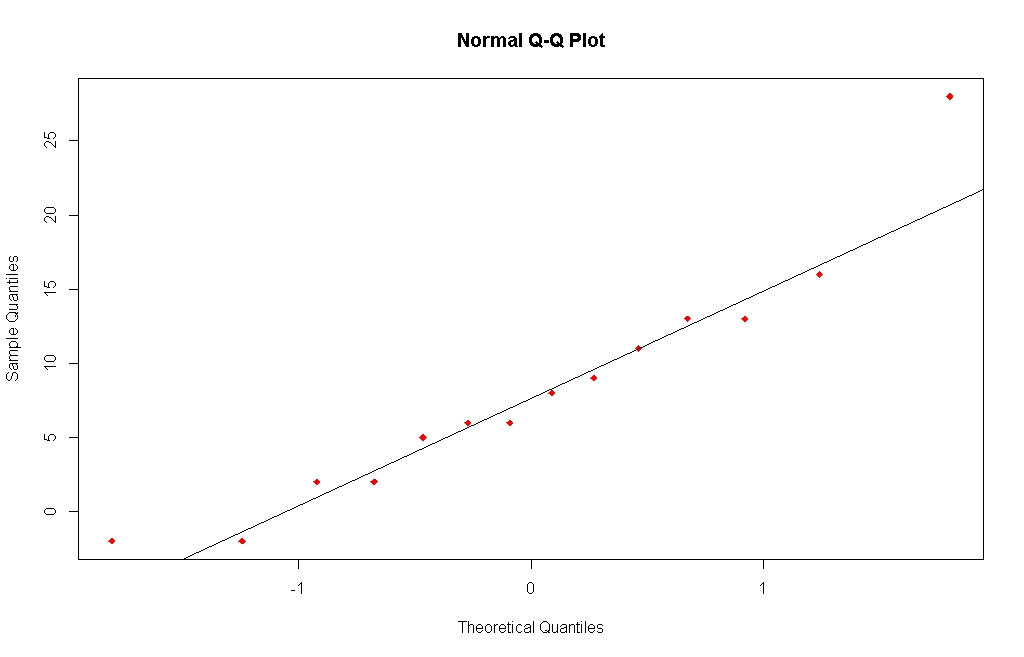
\includegraphics[scale=0.38]{10AQQplot}
\end{center}


\end{itemize}
\end{document}